%\bookmarksetup{startatroot}
\appendixtitleon
\appendixtitletocon
\begin{appendices}
%\addtocontents{toc}{\protect\setcounter{tocdepth}{0}}
%\appendix
%\clearpage
\vspace*{\stretch{2}}%{\fill}
\begin{center}
\begin{minipage}{.75\textwidth}
\section{Instalación del \emph{hardware} necesario}\label{ApendiceA}


Una vez revisado el análisis previo y funcional del sistema de sensado móvil colaborativo mediante un visión \emph{top-down}, en este capítulo presentamos  el análisis orgánico de la implantación mediante una visión \emph{bottom-up}. Esto es, primero se configura el nivel inferior, la capa del \emph{hardware} y el Control de Red, tras lo cual se va ascendiendo en el modelo hasta llegar a la implantación del portal cautivo, en la capa de Usuarios y el nivel más alto del sistema total.
\end{minipage}
\end{center}
\vspace{\stretch{3}} % \vfill % equivalent to \vspace{\fill}
\clearpage% https://tex.stackexchange.com/questions/70714/center-horizontally-and-vertically-a-block-of-text

En este Apéndice se asume que se dispone de conexión a Internet operativa a la que la Raspberry Pi 3 pueda conectarse (cableada o inalámbrica) y un ordenador de trabajo, no entrando en detalles sobre su configuración por entender que no es parte del TFG.

Para poner en marcha la Raspberry Pi 3 de forma sencilla es necesario disponer de la propia placa, una fuente de alimentación USB Micro (un adaptador de corriente como el de la mayoría de teléfonos móviles actuales), teclado y ratón, una tarjeta microSD de al menos 8 GB clase 4 y un monitor con entrada HDMI, para lo que puede servir una pantalla de televisión. También hace falta disponer de conexión a Internet, ya sea mediante red cableada o una red inalámbrica a la que la Raspberry Pi 3 pueda conectarse.

La tarjeta microSD debe de tener ya almacenado el sistema operativo Raspbian desde el principio o por el contrario hacer uso de la solución recomendada desde la propia página Web oficial, la herramienta \emph{New Out Of Box Software} (\emph{\acrshort{NOOBS}}, que en inglés significa \emph{novatos}). Esta herramienta es un gestor de instalaciones de sistemas operativos para la Raspberry Pi, disponible desde su página Web oficial. Puede comprarse la tarjeta SD con dicha herramienta preinstalada o puede instalarse manualmente haciendo uso de un ordenador, descargando el archivo comprimido de NOOBS y descomprimiéndolo en una tarjeta SD vacía y formateada en FAT32, de forma que los archivos estén en el directorio raíz de la tarjeta. Tras este proceso la tarjeta queda preparada para funcionar insertándose en la Raspberry Pi 3, enchufando la misma al teclado, ratón y monitor y por último a la corriente eléctrica.

Al ser enchufada a la corriente la Raspberry Pi se inicia de forma automática y carga la herramienta NOOBS, tras lo que aparece la pantalla de selección de sistemas operativos en el que debemos seleccionar Raspbian (Figura \ref{NOOBS}) y pulsar el botón \emph{Instalar} en la esquina superior izquierda del menú, tras lo cual comienza el proceso de instalación de Raspbian utilizando la totalidad de la tarjeta microSD para su sistema de archivos (si utilizamos la versión ligera de NOOBS primero se efectúa la descarga del mismo, ya que no vendría incluido en la herramienta). Al terminar, la herramienta avisa y se procede al reinicio del dispositivo.

\begin{figure}[!t]
\begin{center}
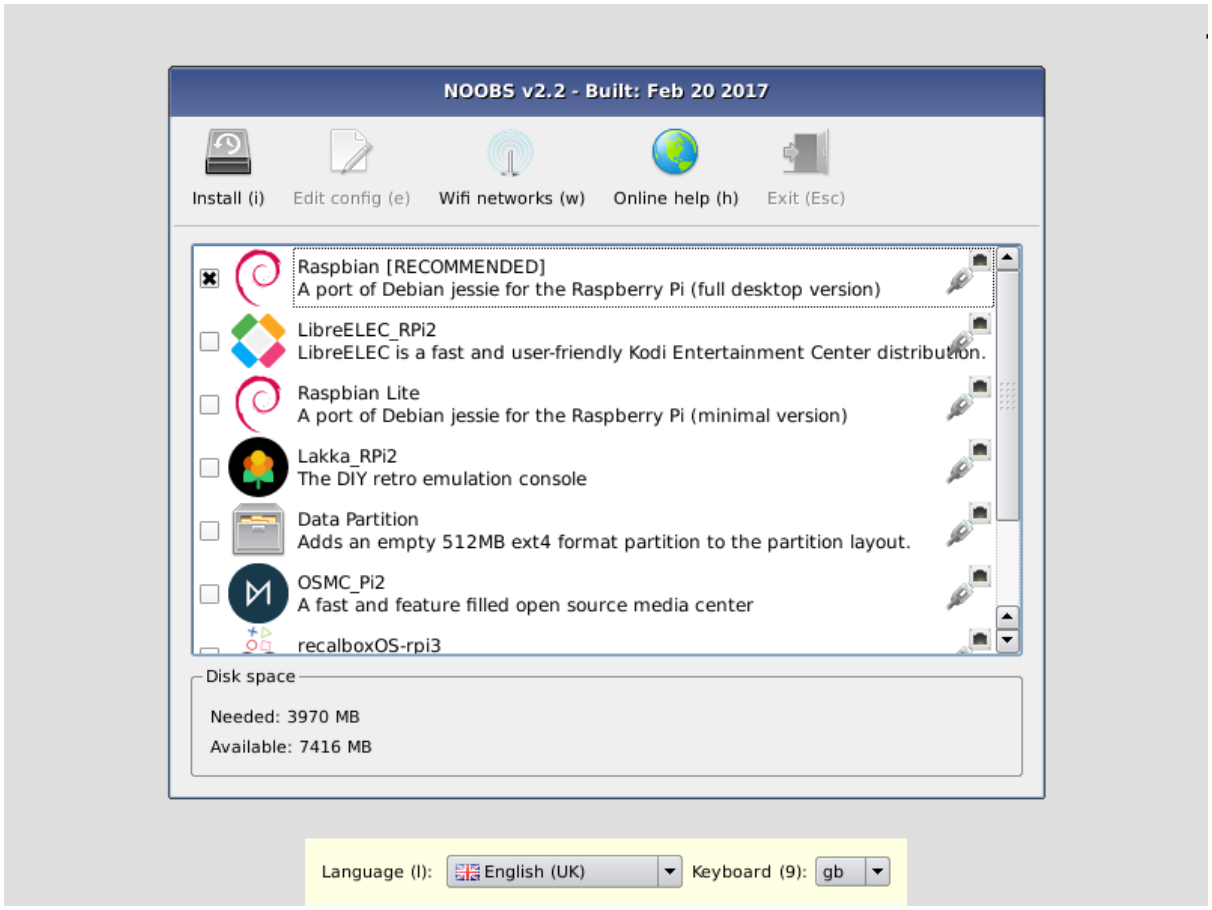
\includegraphics[width=0.75\linewidth]{./X_Anexos/Img/NOOBS.png}
\end{center}
\caption{Selección de Raspbian para ser instalado en la Raspberry Pi 3}
%\source{https://en.wikipedia.org/wiki/RADIUS}
\label{NOOBS}
\end{figure}

Tras la instalación de Raspbian la herramienta NOOBS sigue estando disponible como partición de recuperación para la Raspberry Pi 3, accesible pulsando la tecla \emph{shift} en el momento de encendido al aparecer por primera vez el logotipo de Raspberry Pi.

Aunque su implantación queda fuera del ámbito de este TFG, la Raspberry Pi cuenta con una serie de interfaces activables desde el entorno gráfico o la orden de terminal \emph{raspi-config} que permiten su gestión remota, ya sea mediante \emph{Secure Shell} (\acrshort{SSH}) o servidores \emph{Virtual Network Computing} (\acrshort{VNC}) \cite{RasPiVNC}, tras lo que la Raspberry Pi podría ser manejada en modo headless, sin estar conectada a teclado, ratón o salida de vídeo, tan solo a la corriente y a una red local por medio de alguna de sus interfaces de red.

No entramos en la configuración del hardware de la WiFi de la Raspberry Pi 3 porque ya viene instalada por defecto en Raspbian.

En este apartado no entramos en el detalle de la configuración de \emph{hostapd} porque en el capítulo 5 presentamos toda la instalación del software necesario por orden de dependencias entre ellos, lo cual nos obligaría a explicar previamente aplicaciones que pertenecen a otros módulos.
\cleardoublepage
\vspace*{\stretch{2}}%{\fill}
\begin{center}
\begin{minipage}{.75\textwidth}
\section{Descarga automática del código de la nube}\label{ApendiceB}

Hoy en día la tendencia es a alojar los proyectos de libre distribución y código abierto en la Nube. Nosotros hemos alojado nuestro proyecto en la nube \emph{GitHub}. En este apéndice proporcionamos la dirección Web de acceso a él y la instalación automática de todo el entorno.
\end{minipage}
\end{center}
\vspace{\stretch{3}} % \vfill % equivalent to \vspace{\fill}
\clearpage% https://tex.stackexchange.com/questions/70714/center-horizontally-and-vertically-a-block-of-text

Para implementar el servicio, en lugar de replicar el código manualmente, puede clonarse el repositorio online habilitado explícitamente para ello mediante la herramienta de control de versiones \emph{git}, situándose en el directorio donde se quiera almacenar los archivos y ejecutando la siguiente orden en el terminal: 

\begin{listing}[H]
  \begin{minted}
  [
  frame=lines,
  framesep=2mm,
  baselinestretch=1.2,
  bgcolor=lightgray,
  fontsize=\footnotesize,
  breakanywhere,
  breaklines=true,
  breaksymbolleft={}
  ]
  {bash}
  git clone https://github.com/DavSanchez/CaptivePortal.git
  \end{minted}
\end{listing}

Tras esto, el servicio Web completo puede ponerse en marcha desde este mismo directorio mediante el orden node.

\begin{listing}[H]
  \begin{minted}
  [
  frame=lines,
  framesep=2mm,
  baselinestretch=1.2,
  bgcolor=lightgray,
  fontsize=\footnotesize,
  breakanywhere,
  breaklines=true,
  breaksymbolleft={}
  ]
  {bash}
  node nodeserver.js
  \end{minted}
\end{listing}


\cleardoublepage
\vspace*{\stretch{2}}%{\fill}
\begin{center}
\begin{minipage}{.75\textwidth}

\section{Reanudación automática del servidor en caso de fallo}\label{ApendiceC}

Proporcionando la orden de arranque del Apéndice \ref{ApendiceB} (\emph{node nodeserver.js}) es suficiente para que el sistema de sensado móvil colaborativo arranque y proporcione los servicios desarrollados. sin embargo, se puede dar el caso de fallos del servidor en cuyo caso debemos tolerarlos. En este apéndice se explica como hacerlo.
\end{minipage}
\end{center}
\vspace{\stretch{3}} % \vfill % equivalent to \vspace{\fill}
\clearpage% https://tex.stackexchange.com/questions/70714/center-horizontally-and-vertically-a-block-of-text

La orden ejecutada justo al final del apartado anterior basta para poner en marcha el servicio, pero no protege ante la situación de que un fallo detenga su ejecución y requiere que un administrador lo ejecute siempre que el hardware se pone en marcha. Existen diversas utilidades para solucionar esta situación no deseada; la utilizada en este TFG es PM2.

PM2 es un gestor de procesos para Node.js que nos permite configurar el comportamiento del servicio Web implementado frente a cambios en los archivos locales (como una actualización) u otras situaciones. Puede instalarse a través del gestor de paquetes \emph{npm}:

\begin{listing}[H]
  \begin{minted}
  [
  frame=lines,
  framesep=2mm,
  baselinestretch=1.2,
  bgcolor=lightgray,
  fontsize=\footnotesize,
  breakanywhere,
  breaklines=true,
  breaksymbolleft={}
  ]
  {bash}
  npm install pm2 -g
  \end{minted}
\end{listing}

Tras instalar esta herramienta ejecutaríamos una serie de órdenes con ella que nos permiten reanudar la aplicación Node.js de forma automática nada más encender nuestra Raspberry Pi 3, reiniciando el servicio si ocurre algún error o incluso si actualizamos el código de forma local o remota (editándolo en otra parte, subiéndolo a GitHub y recuperándolo con la orden \emph{git pull}): 

\begin{listing}[H]
  \begin{minted}
  [
  frame=lines,
  framesep=2mm,
  baselinestretch=1.2,
  bgcolor=lightgray,
  fontsize=\footnotesize,
  breakanywhere,
  breaklines=true,
  breaksymbolleft={}
  ]
  {bash}
  pm2 startup
  \end{minted}
\end{listing}

Esta orden detecta el sistema en el que nos encontramos y nos recomienda el orden a ejecutar para generar un \emph{startup script}, que es ejecutado nada más encender el dispositivo. Una salida de ejemplo de este orden es la siguiente:

\begin{listing}[H]
\begin{minted}
[
frame=lines,
framesep=2mm,
baselinestretch=1.2,
bgcolor=lightgray,
fontsize=\footnotesize,
breaklines=true,
breaksymbolleft={}
]
{bash}
[PM2] You have to run this command as root. Execute the following command:
      sudo su -c "env PATH=$PATH:/home/unitech/.nvm/versions/node/v4.3/bin pm2 startup <distribution> -u <user> --hp <home-path>
\end{minted}
\caption{PM2 sugiere un comando a introducir para poder ejecutarse al iniciar el sistema}
\label{startupScript}
\end{listing}

Tras este proceso, solo queda configurar los parámetros a usar por PM2, ejecutar las aplicaciones Node.js deseadas y guardar el entorno con la siguiente orden:

\begin{listing}[H]
  \begin{minted}
  [
  frame=lines,
  framesep=2mm,
  baselinestretch=1.2,
  bgcolor=lightgray,
  fontsize=\footnotesize,
  breakanywhere,
  breaklines=true,
  breaksymbolleft={}
  ]
  {bash}
  pm2 save
  \end{minted}
\end{listing}

Este paso asegura que la aplicación Node.js vuelve a ejecutarse tras un reinicio del sistema, ya sea un reinicio programado o el ocurrido tras un corte accidental.

Para conseguir lo anterior es necesario configurar el entorno de programación. Para ello se puede utilizar un archivo de configuración como el empleado en este TFG, ubicado en la raíz del repositorio de GitHub con el nombre \emph{captiveportalserver.config.js}. El contenido de este archivo es el siguiente:

\begin{listing}[H]
\begin{minted}
[
frame=lines,
framesep=2mm,
baselinestretch=1.2,
bgcolor=lightgray,
fontsize=\footnotesize,
breaklines=true,
breaksymbolleft={}
]
{javascript}
module.exports = {
 apps : [
   {
     name      : "nodeserver",
     script    : "./nodeserver.js",
     watch     : true,
 ignore_watch: ["./.git", "./node_modules", "./.gitignore", "./uploads", "./users/users.json", "./users/usersOneTime.json"]
   }
 ]
}
\end{minted}
\caption{Fichero de configuración del entorno node con PM2}
\label{PM2Env}
\end{listing}

Se observa que se trata esencialmente de un objeto JavaScript con los siguientes campos:

\begin{itemize}
\item \emph{name}: el nombre asignado al proceso.
\item \emph{script}: la ubicación del archivo Node.js que ejecutaríamos normalmente con la orden \emph{node}.
\item \emph{watch}: un flag que vigila cambios en nuestros archivos, reiniciando la aplicación Node.js si se detectara uno.
\item \emph{ignore\_watch}: \emph{Array} de archivos y directorios que no se vigilan con el \emph{flag} anterior.
\end{itemize}

Si nuestro entorno requiriese de más aplicaciones Node.js ejecutadas simultáneamente podrían añadirse como nuevas instancias del objeto \emph{apps}.

Una vez terminada la configuración de nuestro entorno, lo ejecutamos mediante PM2 (no mediante node) y guardamos el entorno tal y como se nos queda para que se ejecute de la siguiente forma cada vez que se inicie nuestro sistema.

\begin{listing}[H]
  \begin{minted}
  [
  frame=lines,
  framesep=2mm,
  baselinestretch=1.2,
  bgcolor=lightgray,
  fontsize=\footnotesize,
  breakanywhere,
  breaklines=true,
  breaksymbolleft={}
  ]
  {bash}
pm2 start captiveportalserver.config.js
pm2 save
  \end{minted}
\end{listing}

Por último, con la orden \emph{pm2 monit} puede accederse a una vista de monitorización que nos permite ver una lista de las aplicaciones activas y su consumo en memoria, la salida en consola de cada una de ellas, el número de veces que se han reiniciado (Figura \ref{pm2monit}).

\begin{figure}[!t]
\begin{center}
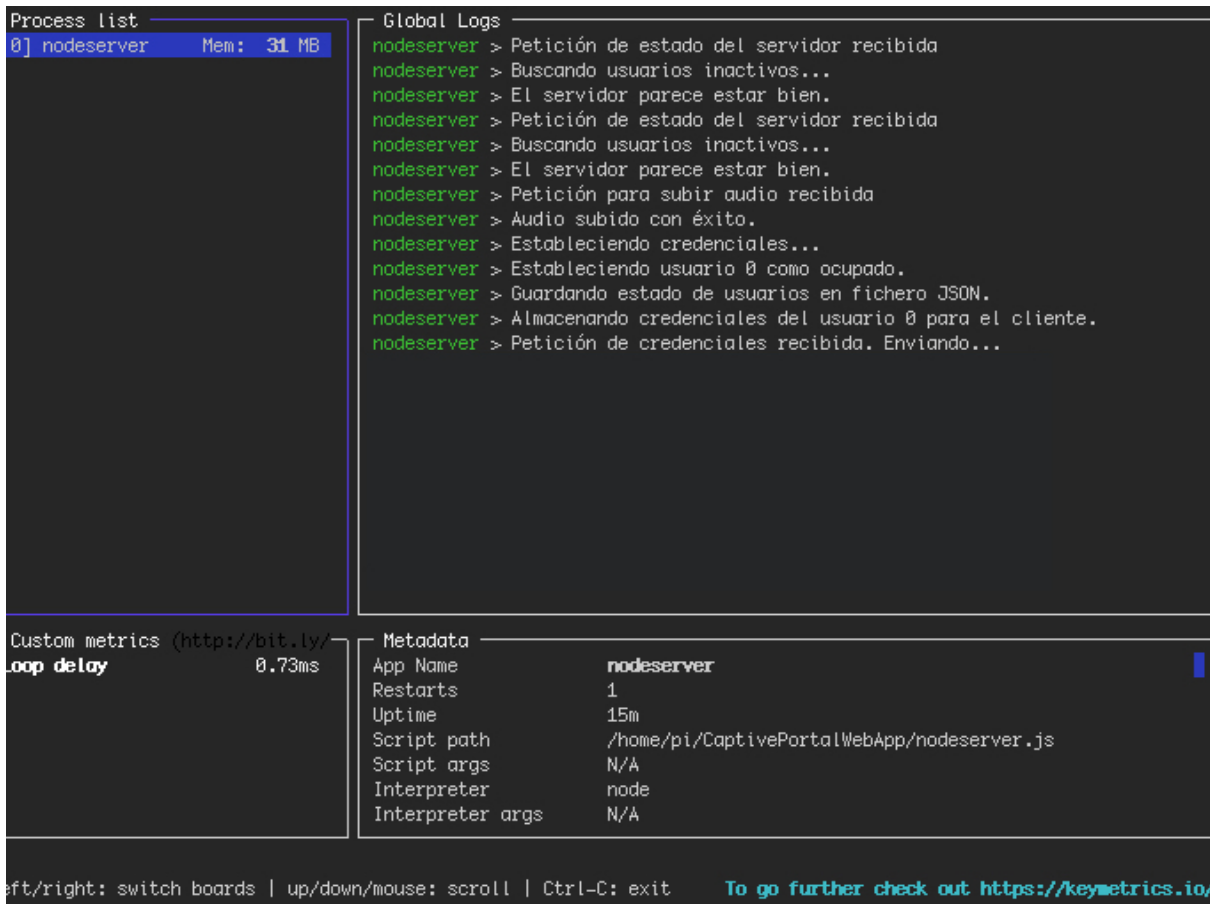
\includegraphics[width=0.75\linewidth]{./X_Anexos/Img/pm2monit.png}
\end{center}
\caption{Vista de monitorización de aplicaciones activas con pm2 monit}
%\source{https://en.wikipedia.org/wiki/RADIUS}
\label{pm2monit}
\end{figure}
\cleardoublepage
\vspace*{\stretch{2}}%{\fill}
\begin{center}
\begin{minipage}{.75\textwidth}
\section{Ciclo de vida del TFG}\label{ApendiceD}

En este apéndice se presenta una visión rápida del ciclo de vida del TFG. El objetivo es mostrar cómo ha ido evolucionando la implantación del sistema de sensado.
\end{minipage}
\end{center}
\vspace{\stretch{3}} % \vfill % equivalent to \vspace{\fill}
\clearpage% https://tex.stackexchange.com/questions/70714/center-horizontally-and-vertically-a-block-of-text

El desarrollo de este TFG no consistió en considerar un único curso de acción y desarrollar la solución. Durante las etapas iniciales se tuvieron en cuenta e investigaron varias alternativas con el objetivo de llegar al mismo resultado final, elementos que se vieron reflejados en los mecanismos de seguimiento presentados. A continuación detallamos algunos de estas primeras aproximaciones y se explica el motivo de haberlas declinado en favor del camino finalmente escogido.

La primera solución propuesta para el TFG, apareciendo así en la primera versión de la propuesta o anteproyecto, consistía en programar una aplicación nativa para terminales Android que gestionara la captura del audio y la ubicación, habilitando el acceso a Internet una vez transferidos los archivos al servidor. Esta solución podría extenderse más adelante a sistemas iOS. Se pensó también implementar una aplicación universal mediante un \emph{wrapper} como \emph{Apache Cordova}, la tecnología anteriormente conocida como \emph{PhoneGap}, con lo que con una sola programación se podrían obtener aplicaciones para diversos sistemas móviles.

Sin embargo, la propuesta de aplicación nativa resultaba altamente situacional, implicando que un hipotético usuario del servicio tuviera una aplicación instalada en su dispositivo de antemano si quería poder acceder a la red. Además, el desarrollo de aplicaciones nativas orientadas a terminales móviles excluía a los ordenadores portátiles, que sin ser \emph{smartphones} ni \emph{tablets} debían poder utilizar el servicio sin problema. Este enfoque requeriría entonces programar aplicaciones de escritorio separadas o implementar alguna otra solución específica para ellos, lo que alargaría el proceso de programación.

Finalmente, con el objetivo de facilitar lo más posible la implementación y el acceso al servicio, junto a la oportunidad de utilizar tecnologías de aparición reciente como las API de \emph{WebRTC}, se optó por desarrollar una aplicación web, accesible desde cualquier dispositivo que cuente con un navegador compatible.

Para implementar el servidor se pensó desde el primer momento en utilizar la Raspberry Pi. Pese a que se disponía de unas cuantas en su modelo 2 y se intentó implementar en ellas, estas carecen de \emph{chipset} WiFi propio, por lo que se debía adquirir por separado, conectarse a esta por USB y compilar el controlador del \emph{hardware} utilizado. Además, no todos los dispositivos WiFi externos disponibles soportan trabajar en modo punto de acceso indispensable para nuestro proyecto, por lo que había que tener especial cuidado al adquirir uno de ellos. Con el objetivo de ahorrarnos toda esta problemática se decidió trabajar directamente con la Raspberry Pi 3, que ya incluye \emph{chipset} WiFi 802.11n propio capaz de trabajar en el modo deseado, teniendo además el mismo precio que su modelo predecesor. Al igual que se tuvieron en cuenta varias alternativas para la implementación del lado del cliente, se experimentó con diversas posibilidades para el lado del servidor en la Raspberry Pi hasta optar por la escogida finalmente.

Durante el proceso de documentación, previa a la implementación del TFG se pensó en implantar el control de acceso a la red manualmente. Para ello se contemplaron diversas opciones para servidores DHCP (como \emph{dnsmasq} o \emph{isc-dhcp-server}) que proporcionarían direccionamiento IP a los dispositivos conectados. Junto a estos actuaría la utilidad de Linux \emph{iptables}, que permite establecer reglas para el procesamiento de paquetes IP, pudiendo aplicarse permanentemente a través del paquete \emph{iptables-persistent} o mediante \emph{scripts} que se ejecutarían y aplicarían las reglas al iniciar el sistema operativo. Sin embargo, este último paquete presentó problemas al ser instalado en la Raspberry Pi, por lo que esta opción fue descartada al poco tiempo de descubrir la solución que proporcionaba CoovaChilli.

En cuanto a los servidores Web para alojar el portal cautivo, inicialmente se pensó en utilizar un enfoque tradicional con servidores como \emph{Apache}, \emph{Nginx} o soluciones ligeras como \emph{lighttpd} junto a PHP o \emph{web scripts} CGI. Finalmente fueron parcialmente descartados como implementación principal en favor de tecnologías web de gran popularidad actual como Node.js, usando el servidor web Nginx solamente para alojar la interfaz web daloRADIUS.

Aunque Raspbian es la oficial, la Raspberry Pi permite instalar otras distribuciones y sistemas operativos. Uno de ellos es \emph{OpenWRT}, una solución de código abierto para sistemas empotrados orientados a encaminamiento de tráfico de red. Puede instalarse en pasarelas residenciales, ordenadores portátiles e incluso teléfonos móviles, por lo que su instalación es viable en la Raspberry Pi. OpenWRT tiene disponible una gran cantidad de protocolos como DNS y DHCP, \acrshort{NAT}, mapeo de puertos, aplicaciones de seguridad... También es posible el uso de portales cautivos instalando \emph{CoovaChilli}.

Finalmente se decidió no optar por esta solución debido a que la distribución basada en \emph{Debian} predeterminada para la Raspberry Pi ofrece un soporte más amplio en cuanto a documentación y mayores posibilidades para implementar otras tareas relacionadas con el proyecto: gestión, análisis y procesado de los ficheros de audio, simulaciones de ubicación acústica, etc.

Junto a CoovaChilli se evaluó otra solución de control de acceso a la red disponible para Linux: \emph{PacketFence}. Este programa de código abierto es también muy completo, ofreciendo facilidades de monitorización, análisis de ficheros transmitidos, gestión centralizada tanto cableada como inalámbrica (802.1X) y utilidades de portal cautivo. Lamentablemente, cuando se estudió su uso \emph{PacketFence} no garantizaba compatibilidad total para la Raspberry Pi, por lo que también fue descartado.

\cleardoublepage
\vspace*{\stretch{2}}%{\fill}
\begin{center}
\begin{minipage}{.75\textwidth}
\section{Problemas acontecidos en el desarrollo de la solución}\label{ApendiceE}

En este apéndice se detallan algunas dificultades ocurridas durante el desarrollo del TFG que limitaron el diseño del sistema final y alargaron en el tiempo desarrollos que a priori no tenían dificultad.
\end{minipage}
\end{center}
\vspace{\stretch{3}} % \vfill % equivalent to \vspace{\fill}
\clearpage% https://tex.stackexchange.com/questions/70714/center-horizontally-and-vertically-a-block-of-text

Uno de los problemas a los que nos enfrentamos a la hora de implementar este TFG es el de los navegadores compatibles con WebRTC. La API \emph{MediaStream Recording} utilizada aún no está soportada por todos los navegadores, siendo Safari, navegador de los dispositivos Apple, el ejemplo más relevante de esta falta de soporte. Este problema es mayor de lo que parece debido a que Apple obliga a que todos los navegadores disponibles en la App Store de iOS hagan uso del motor de renderizado web WebKit que también usa Safari, por lo que en un dispositivo iOS no podemos simplemente cambiar de navegador para que nuestro sistema funcione.

Aunque no presenta problema a la hora de ser probado en local, las API de geolocalización y de grabación multimedia requieren de un contexto seguro. Esto implica que el sistema no funciona sin hacer uso de HTTPS, por lo que hubo que implementar este sistema en nuestra aplicación web haciendo uso de la herramienta OpenSSL, la API correspondiente para \acrshort{HTTPS} en Node.js y habilitar esta opción en CoovaChilli.

Dado que OpenSSL genera certificados auto-firmados, y por tanto no reconocidos por una autoridad de certificación, los navegadores no los aceptan de primeras para proteger al usuario, por lo que a efectos de hacer las pruebas hubo que añadir las excepciones de la aplicación web y la interfaz JSON de \emph{CoovaChilli} manualmente.

\cleardoublepage
\vspace*{\stretch{2}}%{\fill}
\begin{center}
\begin{minipage}{.75\textwidth}
\section{Desarrollo temporal}\label{ApendiceF}

Se presenta una tabla de desarrollo temporal.
\end{minipage}
\end{center}
\vspace{\stretch{3}} % \vfill % equivalent to \vspace{\fill}
\clearpage% https://tex.stackexchange.com/questions/70714/center-horizontally-and-vertically-a-block-of-text

La cronología de desarrollo aproximado del proyecto se muestra en la Tabla \ref{tablaTFG}.

\begin{table}[!ht]
\begin{center}
\begin{tabular}{ | l | c | }
\hline
\textbf{Tarea acometida} & \textbf{Tiempo invertido} \\
\hline
Documentación inicial & 10 horas \\ \hline
Especificación & 10 horas \\ \hline
Opciones consideradas & 10 horas \\ \hline
Análisis software de servidor & 20 horas \\ \hline
Diseño final & 20 horas \\ \hline
Implementación final (WebApp + Server) & 160 horas \\ \hline
Pruebas en Raspberry Pi 2 + Interfaz WiFi & 5 horas \\ \hline
Configuración de Seguridad HTTPS & 5 horas \\ \hline
Pruebas en Raspberry Pi 3 & 10 horas \\ \hline
Correcciones y cambios & 20 horas \\ \hline
Pruebas finales & 20 horas \\ \hline
Elaboración de documentos finales & 10 horas \\ \hline
\end{tabular}
\end{center}
\caption{Cronología aproximada de realización del TFG}
\label{tablaTFG}
\end{table}%

\end{appendices}